\subsection{Database}
The database will be used to keep track of user info which includes name, email, passwords, connections [to different services], and user preferences.

\begin{figure}[h!]
	\centering
 	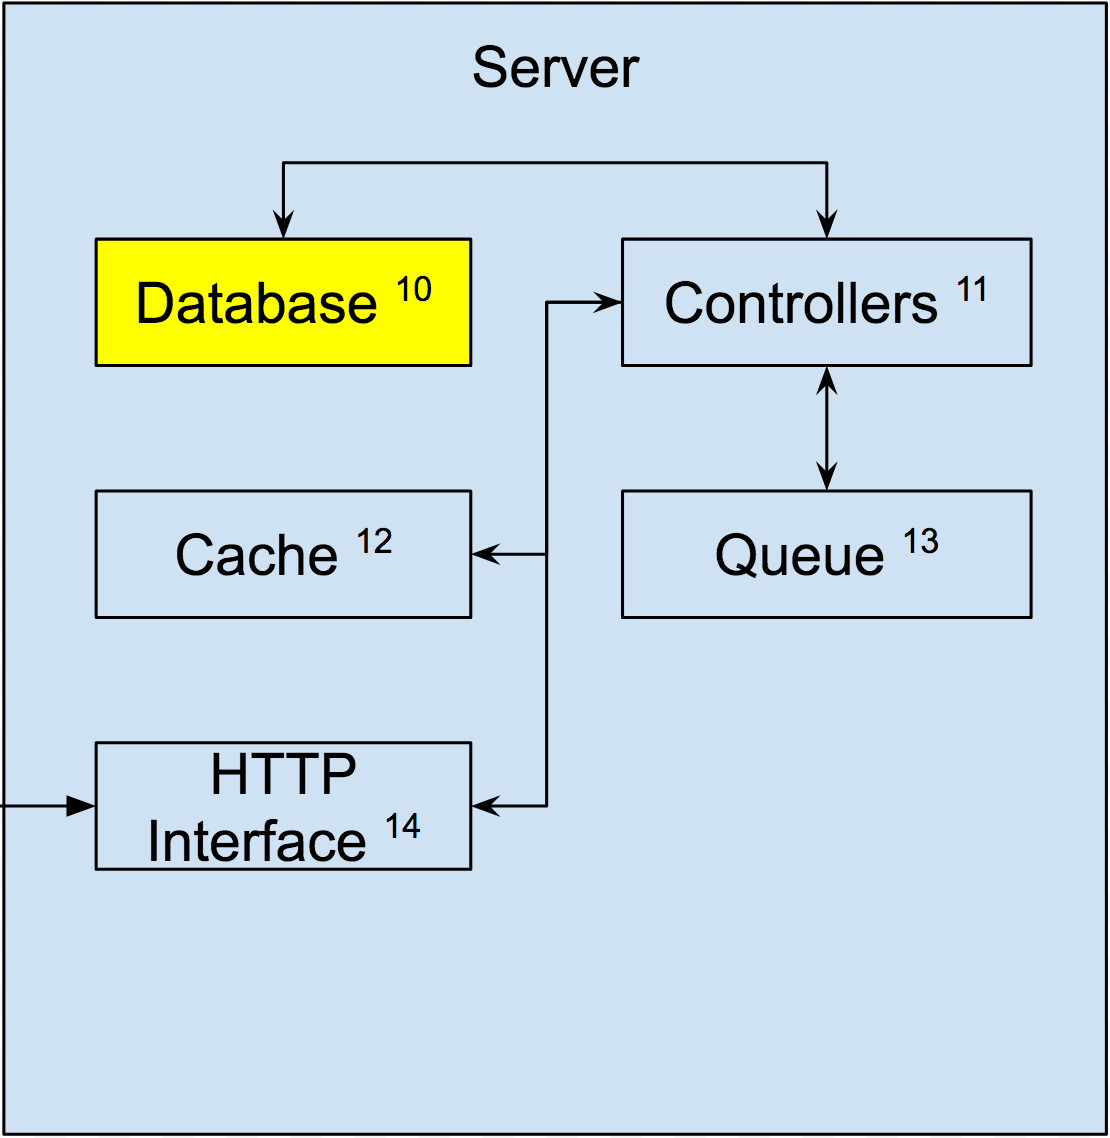
\includegraphics[width=0.60\textwidth]{images/server/server_database.png}
 	\caption{Database subsystem}
\end{figure}

\newpage

\subsubsection{Subsystem Hardware}
This project is primarily software, but we will be hosting our live site using Heroku, so whatever hardware they are using for their servers is our hardware. \\

\subsubsection{Subsystem Operating System}
This project is primarily software, but we will be hosting our live site using Heroku, so whatever OS they are using for their servers (usually UNIX systems such as macOS, Linux) is our OS. \\

\subsubsection{Subsystem Software Dependencies}

Libraries \\
- PostgreSQL \\
- jwt \hspace{3.2cm} "github.com/dgrijalva/jwt-go" \\
- bcrypt \hspace{2.7cm} "golang.org/x/crypto/bcrypt" \\
- pq (postgres driver) \hspace{0.45cm} "github.com/lib/pq" \\ \\
Frameworks \\
- spotify \hspace{2.6cm} "github.com/zmb3/spotify" \\

\subsubsection{Subsystem Programming Languages}
The database interaction models are written in Go, but we are using PostgreSQL under the hood. \\

\subsubsection{Subsystem Data Structures}
We have a User object that will represent a user. Information includes name, email, and password. We also keep track of other attributes on our own in the back-end (when the user was created, the last time any attribute of a user was updated, and access tokens for accessing the API for each platform.) \\

\subsubsection{Subsystem Data Processing}
Once a user has signed in to the service, their information from their connected services will be used to fetch information from each respective service. Stored access tokens will be sent from the database and server, to the client as cookies (which are basically key,vaue pairs). So Hash maps will be the primary data structure

\newpage